\chapter{Case study and experimental setup}
	L'elaborato è stato condotto sfruttando due sistemi differenti, aventi ruolo di \emph{client} e \emph{server}.\par
	Il client ha un processore \texttt{Intel Celeron N3050} $1.60GHz$,  memoria di $4GB$ ed un sistema operativo \texttt{Ubuntu 18.04.1 LTS}.\par
	Il server è costituito da una macchina virtuale con sistema operativo \texttt{Trisquel-mini 8.0}, distribuzione di \emph{GNU} con kernel \emph{Linux-libre}, memoria di $512GB$, risiedente su un sistema con processore \texttt{Intel Core i3} $2.27GHz$.\par
	Il web server utilizzato è \emph{Apache Web Server} versione 2, il load generator \emph{Apache JMeter 5.0}. Esso consente l'invio di richieste HTTP al server con tasso impostabile. La scelta delle pagine su cui incentrare l'esperimento è stata dettata da una ricerca sul web delle dimensioni di quelle, a nostro parere, maggiormente rappresentative: social network, e-commerce, blog, siti aziendali, wiki. Infine abbiamo sfruttato per la scelta il report di \emph{HTTP Archive} sullo stato del web. Esso, infatti, evidenzia come le pagine web, in contesto desktop e mobile, stiano aumentando di dimensioni, passando dalle centinaia di $KB$, al $MB$.
	\begin{figure}[H]
		\centering
		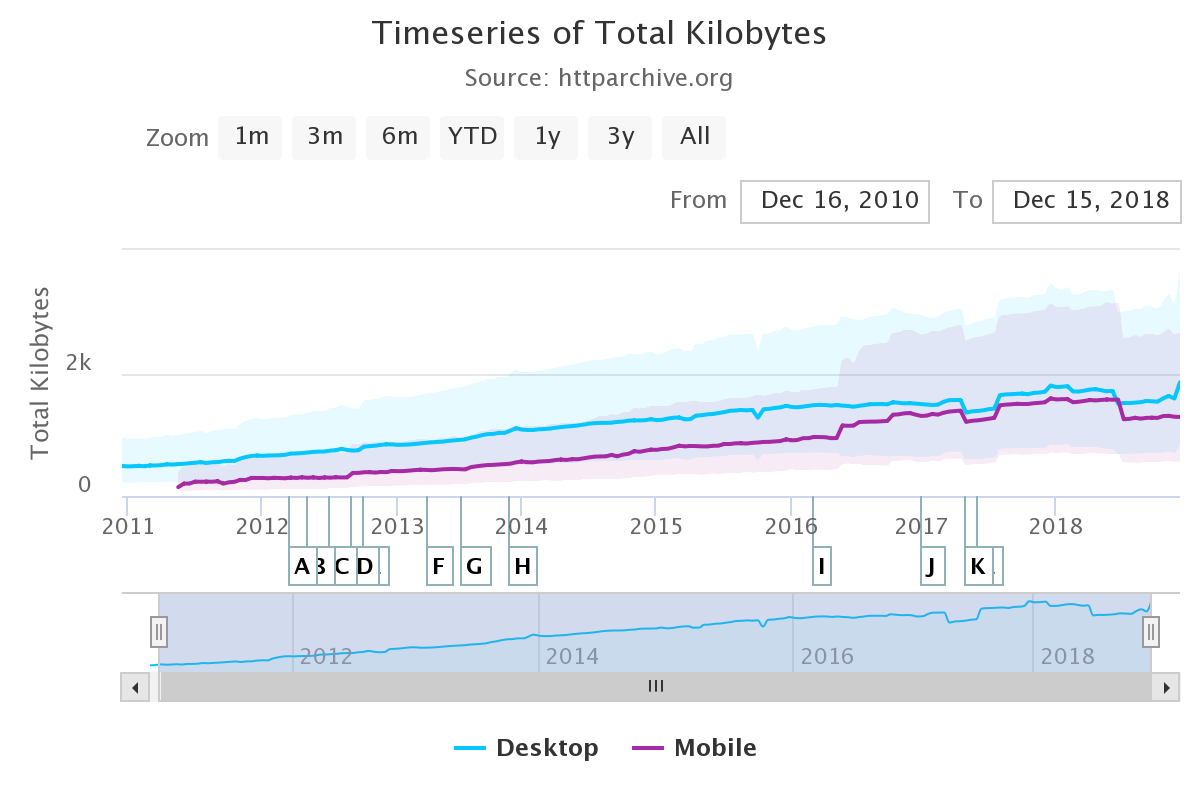
\includegraphics[scale=0.3]{./immagine/chart.png}
		\caption{Stato del Web: Kilobyte totali}
		\label{fig:httparc}
	\end{figure}
	
	\section{Workload Characterization}
		Mediante Jmeter, sono state inviate al server $60req/s$ di 5 diversi tipi di pagine. Il tasso di richieste è stato impostato con il \emph{Constant Throughput Timer}, selezionando $3600req/min$, svolte dai thread complessivamente. Le richieste sono infatti eseguite da 30 thread per 5 minuti. Ogni richiesta può essere casualmente di uno dei 5 tipi:
		\begin{itemize}
			\item \emph{Instagramlogin.html} di $29KB$
			\item \emph{FrancoCFA.html} di $112KB$
			\item \emph{Amazon.html} di $460KB$
			\item \emph{Facebook.html} di $1.4MB$
			\item \emph{Sample-jpg-image-5mb.jpg} di $5MB$
		\end{itemize}
		
		I dati di application level sono stati raccolti con un \emph{Simple Data Writer}. Lato server i dati system level sono stati collezionati per 6 minuti, tramite il comando \textsf{vmstat -n -a 1 360}. Alcune istanze, quindi, tra questi sono precedenti e successive all'esperimento.
		
		\subsection{WL Dati Application Level}
		Nei 5 minuti di test sono state prelevate 515 istanze (richieste inviate al web server) descritte da 17 parametri app-level. Tra questi, quelli maggiormente significativi sono: 
		\begin{itemize}
			\item \textit{Elapsed}: tempo tra la richiesta e l'ultima risposta
			\item \textit{Label}: tipologia di pagina in base alla sua dimensione
			\item \textit{ThreadName}: thread a cui è stata assegnata la richiesta
			\item \textit{Success}: esito della richiesta
			\item \textit{Bytes}: dimensione della pagina richiesta
			\item \textit{Latency}: tempo tra la richiesta e la prima risposta
			\item \textit{Connect}: tempo necessario ad instaurare la connessione
		\end{itemize}
		
		Notando l'andamento delle distribuzioni di questi parametri, si è concluso che ha senso caratterizzare statisticamente solo tre di questi, ovvero \textit{Elapsed}, \textit{Latency} e \textit{Connect}.
		
		\begin{figure}[H]
			\centering
			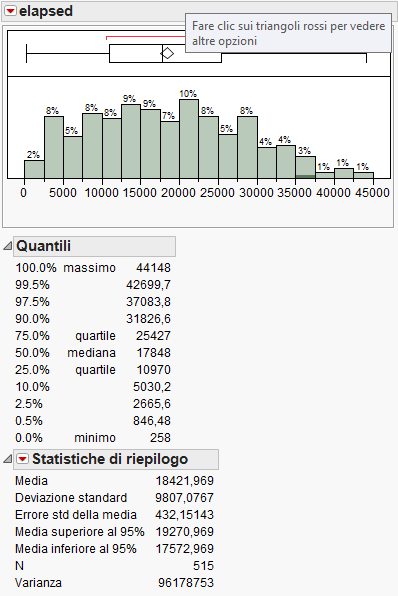
\includegraphics[scale=0.6]{./immagine/elapsed.png}\quad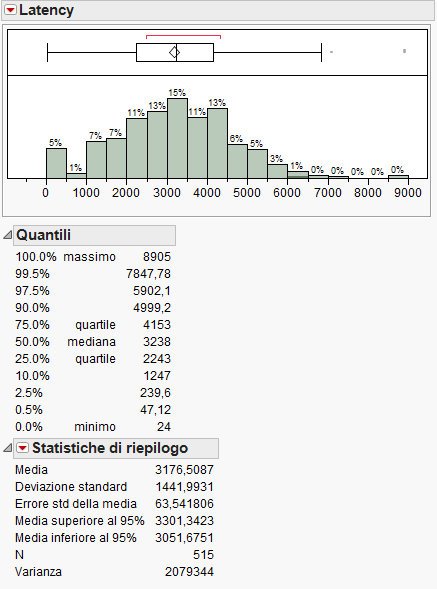
\includegraphics[scale=0.6]{./immagine/latency.png}
			\caption{Distribuzione Elapsed Time e Latency}
			\label{fig:elapse_latency}
		\end{figure}
		
		\begin{figure}[H]
			\centering
			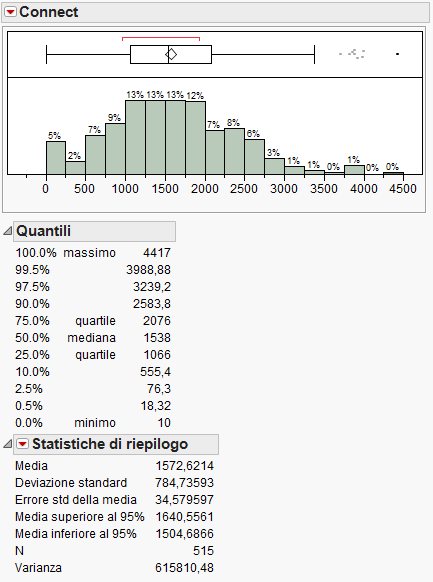
\includegraphics[scale=0.585]{./immagine/connect.png}
			\caption{Distribuzione Connect}
			\label{fig:connect}
		\end{figure}
		
		Osservando le distribuzioni di questi tre parametri, si nota che sono molto poco skewed, quindi si è concluso che la media è un buon indice statistico in grado di descriverle.\\
		Consideriamo ora la distribuzione del parametro \textit{Success}:
		\begin{figure}[H]
			\centering
			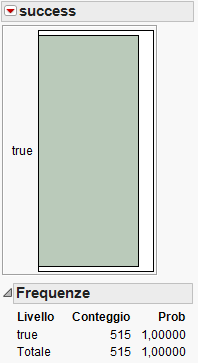
\includegraphics[scale=0.755]{./immagine/success.png}
			\caption{Distribuzione Success}
			\label{fig:success}
		\end{figure}
		
		Come si nota, tutte le richieste sono andate a buon fine il che 	vuol dire che la connessione è molto affidabile e nel nostro caso non ha generato mai un fallimento.Questo è dovuto al fatto che si è utilizzata una connessione Ethernet che dal punto di vista fisico è molto affidabile, così come il protocollo applicativo http eseguito dalle richieste, poiché si basa su TCP.\\\\\\
		Osserviamo ora la distribuzione dei parametri \textit{Label} e \textit{ThreadName}:
		
		\begin{figure}[H]
			\centering
			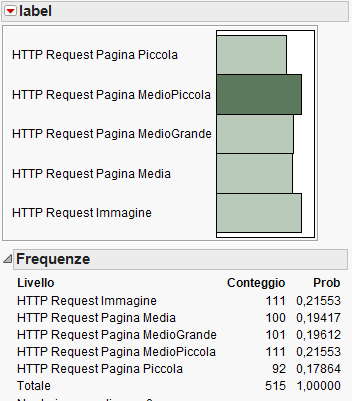
\includegraphics[scale=0.7]{./immagine/label.png}\quad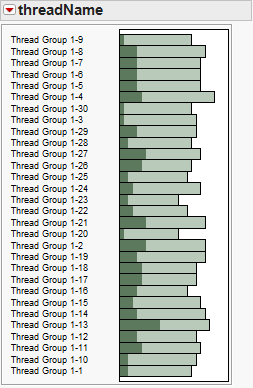
\includegraphics[scale=0.96]{./immagine/threadname.png}
			\caption{Distribuzione Label e ThreadName}
			\label{fig:label_threadname}
		\end{figure}
		
		
		Come si nota ogni tipologia di pagina è distribuita abbastanza equamente tra i thread, per una distribuzione del carico alquanto regolare.\\\\
		Infine si è deciso di verificare come variano i parametri \textit{Elapsed}, \textit{Latency} e \textit{Connect} al variare della dimensione delle pagine richieste.
		
		\begin{figure}[H]
			\centering
			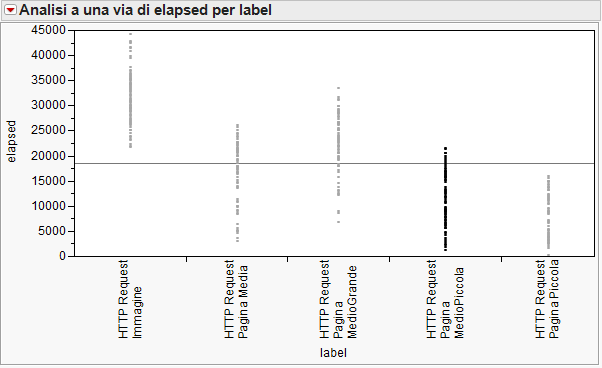
\includegraphics[scale=0.85]{./immagine/grafico_elapsed.png}
			\caption{Grafico variazione Elapsed rispetto alla tipologia di pagina}
			\label{fig:grafico_elapsed}
		\end{figure}
		
		Come si nota dalla \textbf{Figura \ref{fig:grafico_elapsed}}, l'elapsed time cresce al crescere della dimensione delle pagine (misurata in bytes).\\
		Di seguito invece gli altri due grafici mostrano come latency e tempo di connessione non dipendano dalla grandezza delle pagine.
		
		\begin{figure}[H]
			\centering
			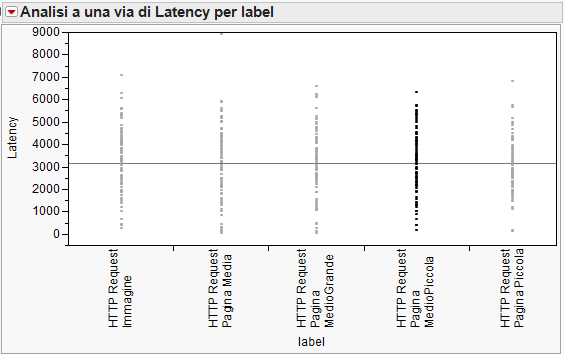
\includegraphics[scale=0.85]{./immagine/grafico_latency.png}
			\caption{Grafico variazione Latency rispetto alla tipologia di pagina}
			\label{fig:grafico_latency}
		\end{figure}
		
		\begin{figure}[H]
			\centering
			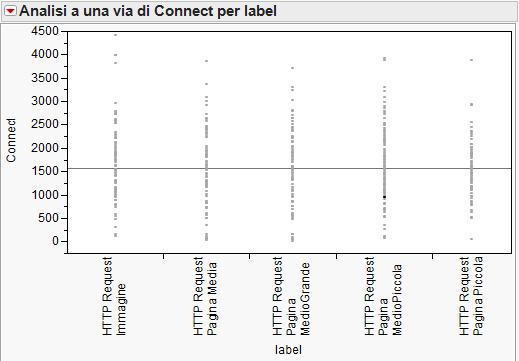
\includegraphics[scale=0.85]{./immagine/grafico_connect.png}
			\caption{Grafico variazione Connect rispetto alla tipologia di pagina}
			\label{fig:grafico_connect}
		\end{figure}
		
		Tutto quello appena detto si può verificare anche calcolando la correlazione tra i parametri elapsed, latency, bytes e connect. Calcoliamo quindi la matrice di correlazione:\\
		
		\begin{figure}[H]
			\centering
			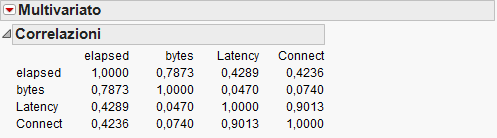
\includegraphics[scale=0.85]{./immagine/correlazione.png}
			\caption{Matrice di correlazione}
			\label{fig:correlazione}
		\end{figure}
		
		Si può vedere come elapsed e bytes siano molto correlati a differenza degli altri parametri, questo perché più è grande la pagina richiesta in termini di byte, più è grande il tempo di risposta.\\\\
		
		\subsection{WL Dati System Level}
		Passiamo all'analisi dei dati di basso livello del sistema. Nei 5 minuti in cui è stato eseguito il test, sono stati prelevate 360 istanze (una al secondo) descritte da 17 parametri. Di queste sono state eliminate le prime tre e le ultime 26 perché precedenti e successive all'esperimento così come si nota dal corrispondente basso numero di interruzioni e dall'alta percentuale di tempo in cui il sistema è idle.\\
		Per prima cosa osservando le distribuzioni dei parametri, sono state eliminate le colonne a varianza nulla che sono 6. Sulle colonne rimaste applichiamo la tecnica della PCA per trovare le componenti principali.
		
		\begin{figure}[H]
			\centering
			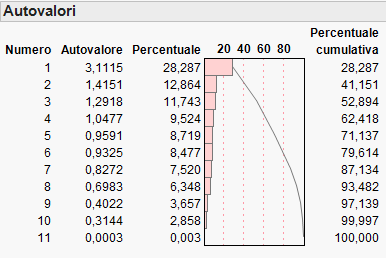
\includegraphics[scale=0.85]{./immagine/autovalori_ex3.png}
			\caption{Componenti principali e varianza conservata}
			\label{fig:autovalori_ex3}
		\end{figure}
		
		Osservando gli autovalori, si è scelto di prendere 9 componenti principali che spiegano il 97\% della varianza.\\
		Dopo aver fatto questo, si adotta la tecnica di clustering di Ward sulle 9 componenti per ridurre il numero di istanze del dataset originario. Osservando il dendrogramma si è determinato che il salto si trovasse a 17 cluster, che determinano una perdita di varianza pari al 30\%, permettendo quindi di conservarne il 70\%.
		
		\begin{figure}[H]
			\centering
			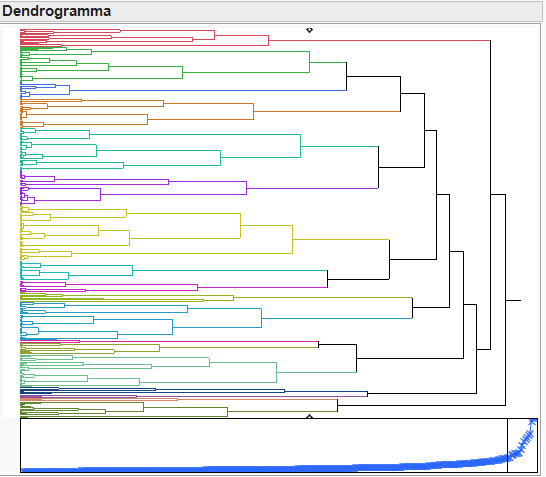
\includegraphics[scale=0.85]{./immagine/dendrogramma_ex3.png}
			\caption{Dendrogramma}
			\label{fig:dendrogramma_ex3}
		\end{figure}
		
		Infine riportiamo l'insieme di istanze rappresentative del dataset oroginario, selezionate in maniera casuale prendendone una per ogni cluster. 
		
		\begin{figure}[H]
			\centering
			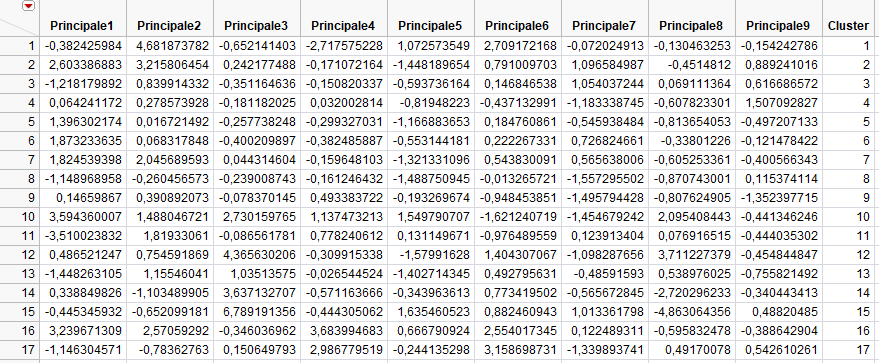
\includegraphics[scale=0.685]{./immagine/final_data_ex3.png}
			\caption{Dati finali}
			\label{fig:final_data_ex3}
		\end{figure}
		
		
	\section{Capacity Test}
		Il Capacity Test è stato eseguito con le pagine Amazon.html, Facebook.html, Sample-jpg-image-5mb.jpg, rappresentanti tipologie di pagine piccole, medie e grandi. Il test è stato attuato prima considerando tutte le pagine (\emph{Random Controller}), poi ciascuna singolarmente.\par
		Throughput e response time sono stati analizzati al crescere delle richieste al minuto. Diverse osservazioni sono state collezionate per una singola condizione di carico, caratterizzate, poi, dalla media, poiché c'è interesse nell'andamento globale.\par
		Il tasso di richieste desiderato è stato ottenuto stabilendo il tasso per ciascun thread ed incrementando ogni volta il loro numero.
		
		\begin{table}[H]
			\footnotesize
			\caption{Capacity Test per tipo di richiesta}
			\label{tab:ct-tip}
			\centering
			\begin{tabular}{cp{0.5\textwidth}c}
				\toprule
				\textbf{Tipo} &
				\textbf{Usable Capacity} &
				\textbf{Knee Capacity}\\
				\midrule
				Random &
				120 &
				50\\
				\midrule
				Piccola &
				600 &
				200\\
				\midrule
				Media &
				220 &
				88\\
				\midrule
				Grande &
				80 &
				20\\
				\bottomrule			
			\end{tabular}
		\end{table}
	
		I risultati ottenuti sono riportati in \textbf{Tabella \ref{tab:ct-tip}}. Di seguito l'andamento di throughput (1/min) e response time (ms), all'aumentare del carico nei 4 casi considerati.
		
		\begin{figure}[H]
			\centering
			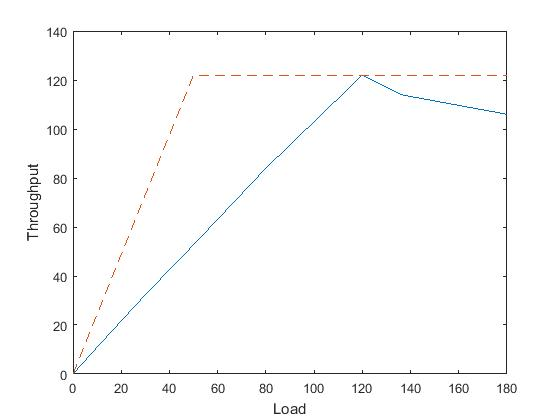
\includegraphics[scale=0.6]{./immagine/randomT.jpg}
			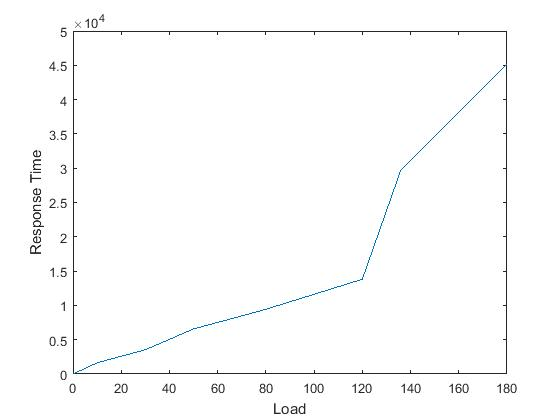
\includegraphics[scale=0.6]{./immagine/randomR.jpg}
			\caption{Pagine Random}
			\label{fig:ct-r}
		\end{figure}
		\begin{figure}[H]
			\centering
			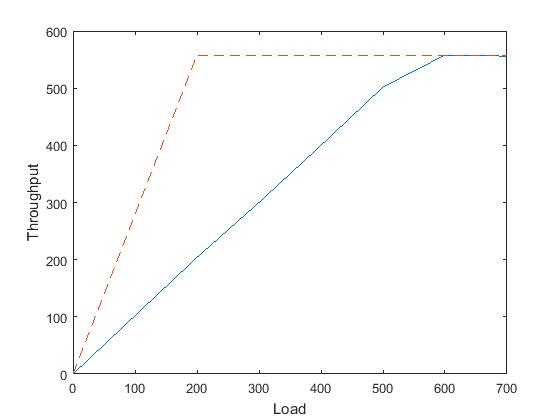
\includegraphics[scale=0.6]{./immagine/piccolaT.jpg}
			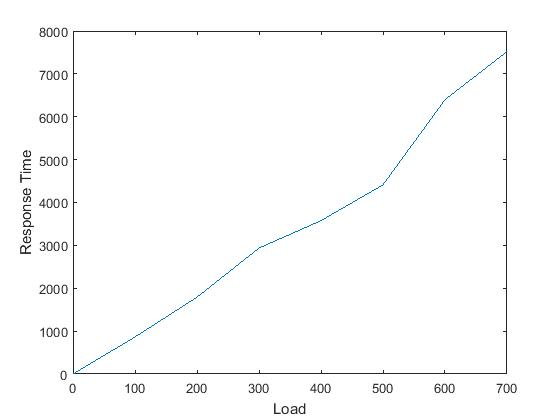
\includegraphics[scale=0.6]{./immagine/piccolaR.jpg}
			\caption{Pagine Piccole}
			\label{fig:ct-p}
		\end{figure}
		\begin{figure}[H]
			\centering
			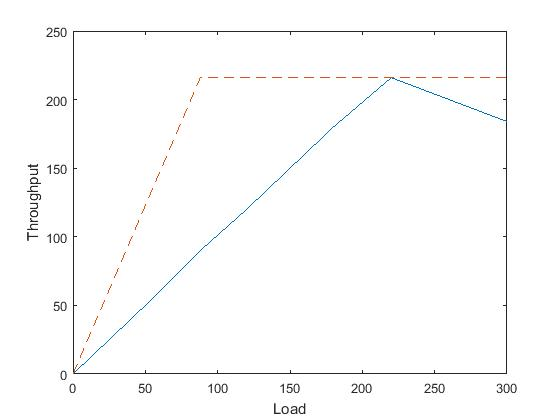
\includegraphics[scale=0.6]{./immagine/mediaT.jpg}
			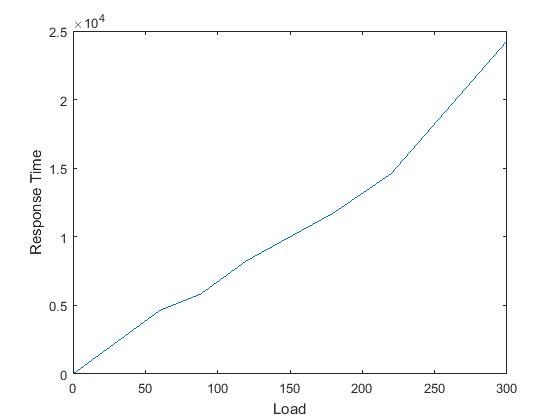
\includegraphics[scale=0.6]{./immagine/mediaR.jpg}
			\caption{Pagine Medie}
			\label{fig:ct-m}
		\end{figure}
		\begin{figure}[H]
			\centering
			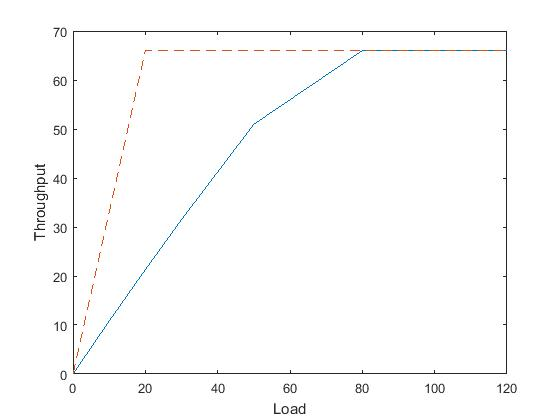
\includegraphics[scale=0.6]{./immagine/grandeT.jpg}
			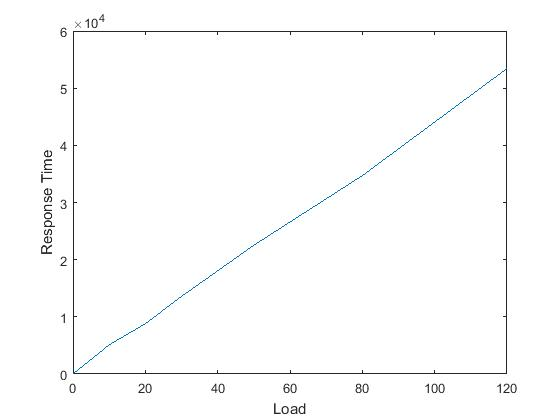
\includegraphics[scale=0.6]{./immagine/grandeR.jpg}
			\caption{Pagine Grandi}
			\label{fig:ct-g}
		\end{figure}
	
		Infine possiamo ricavare i valori per il caso medio ed il caso peggiore delle 3 tipologie di pagine (\textbf{Tabella \ref{tab:ct}}). Osserviamo come il caso medio presenti valori superiori agli altri, poiché molto influenzato dal peso delle pagine piccole. Esse rappresentano la maggioranza delle pagine web di dimensione di centinaia di $KB$, escluse quelle relative ai social network, e non riescono a saturare velocemente il server.
		
		\begin{table}
			\footnotesize
			\caption{Capacity Test}
			\label{tab:ct}
			\centering
			\begin{tabular}{cp{0.5\textwidth}c}
				\toprule
				\textbf{Case} &
				\textbf{Usable Capacity} &
				\textbf{Knee Capacity}\\
				\midrule
				Random &
				120 &
				50\\
				\midrule
				Average &
				300 &
				102.7\\
				\midrule
				Worst &
				80 &
				20\\
				\bottomrule			
			\end{tabular}
		\end{table}
	
	\section{Experimental Design and Analysis}
		Per studiare l'impatto del tasso di richiesta e del tipo di pagina sul tempo di risposta medio, si prosegue con la tecnica del \emph{Design of Experiment}. I fattori sono stati categorizzati. Si sono considerati 2 tipi di pagina: Piccola (Amazon.html), Grande (Sample-jpg-image-5mb.jpg). Si sono poi determinati 4 livelli per il tasso di richiesta, corrispondenti al 20\%, 40\%, 60\%, 80\% della usable capacity media delle pagine: Low, Low-Medium, High-Medium, High. I trattamenti sono stati ripetuti per 10 volte ed in ordine casuale, con durata di 1 minuto ciascuno. Tramite JMP si è ricavata la stima del modello.
		
		\begin{figure}[H]
			\centering
			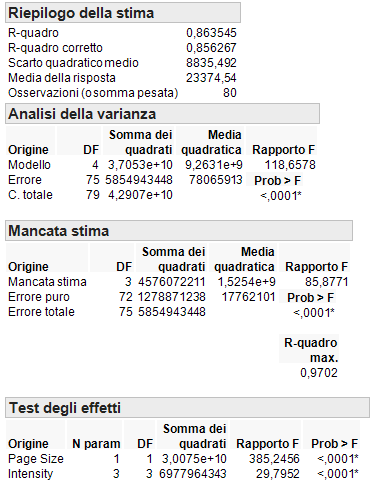
\includegraphics{./immagine/Stimamodello1.png}
			\label{fig:doe-st}
			\caption{Analisi della varianza}
		\end{figure}
	
		Dal rapporto della somma dei quadrati dei fattori rispetto a quella totale, si evince la loro importanza: 70\% della variazione totale è attribuito a Page Size, 16.3\% ad Intensity, il resto all'errore. In realtà parte dell'importanza dell'errore è dovuta all'interazione tra i fattori trascurata, che rappresenta il 10.7\% della variazione totale. Il modello, quindi, spiega circa 86.3\% di SST, come testimonia anche $R^2$.\par
		Per la scelta del tipo di analisi, si provano le assunzioni di normalità ed omoschedasticità. Per la normalità si effetua il \emph{Quantile-Quantile plot} dei residui. Si osserva che la loro distribuzione è asimmetrica. Ciò può essere anche confermato dal test di \emph{Shapiro-Wilk}, che restituisce $p<0.05$, rigettando l'ipotesi di normalità.
		
		\begin{figure}[H]
			\centering
			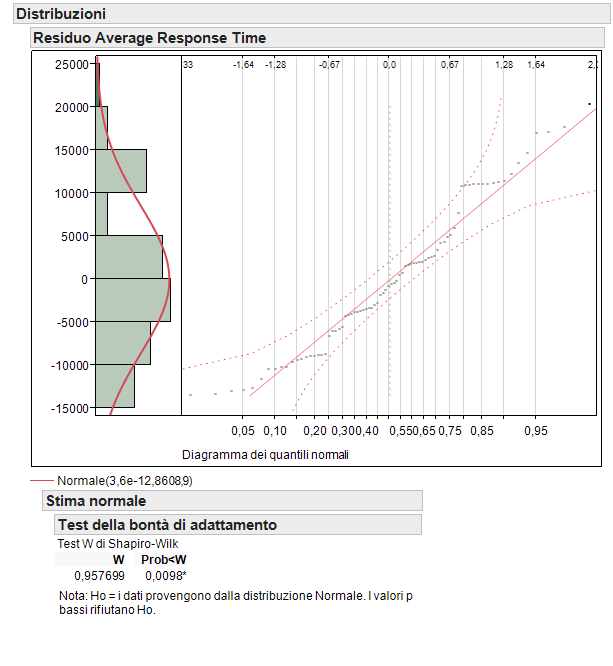
\includegraphics{./immagine/Distribuzione.png}
			\label{fig:doe-n}
			\caption{Q-Q plot e test di Shapiro-Wilk}
		\end{figure}
	
		Necessitiamo, quindi, di un'analisi non parametrica. Ciò può farci già propendere per il test di \emph{Wilcoxon/Kruskal-Wallis}, anche senza valutare l'omoschedasticità (che da test visuale risulta non verificata).
		
		\begin{figure}[H]
			\centering
			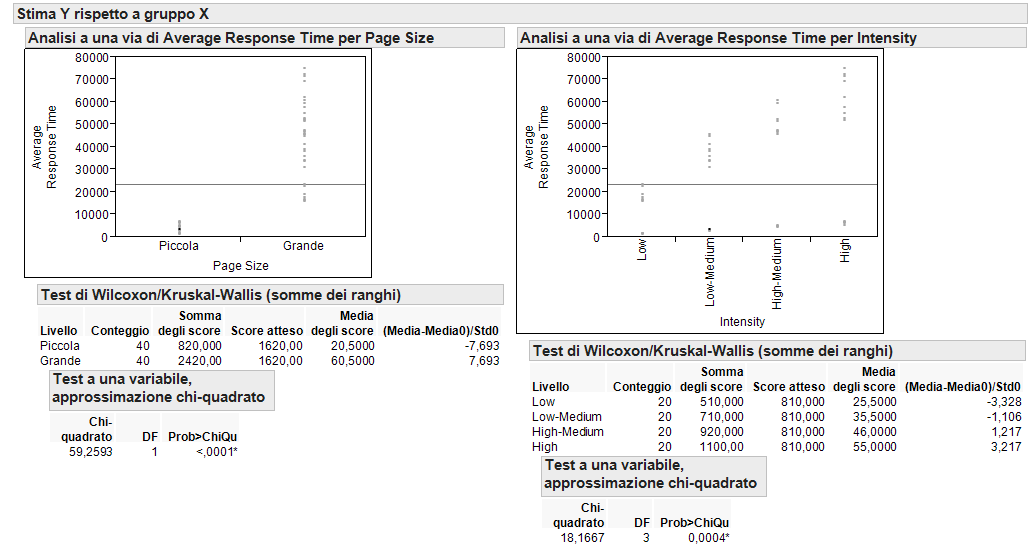
\includegraphics[scale=0.6]{./immagine/StimaYrispettoaX.png}
			\caption{Test di Wilcoxon/Kruskal-Wallis}
			\label{fig:doe-yx}
		\end{figure}
	
		Il test di Kruskal-Wallis rigetta l'ipotesi nulla (campioni dalla stessa popolazione) per entrambi i fattori. Troviamo, infatti, $p<0.05$, quindi entrambi gli effetti sono statisticamente significativi con livello di significatività 0.05.
	